\section{Introduction}
\label{sec: introduction}
The Group Steiner Tree Problem (GSTP) is a classical NP-hard optimization problem. Given a graph with $n$ vertices, $m$ weighted edges, and a query consisting of $g$ groups---each group is a subset of vertices, the goal is to find a tree that contains at least one vertex from each group while minimizing the total edge weight.

% Respond Reviewer #4 R5:The descriptions of the suspendable Dijkstra search and monotonicity-aware pruning could be supplemented with figures to facilitate a more intuitive understanding of these core technical contributions. The authors are encouraged to include illustrative examples of these processes to visualize how the dynamic bounding mechanism and the search space reduction function operate in practice.

% Respond Reviewer #5 R3: The revision should add a small but concrete example explaining the 2-star construction and the main optimization ideas (e.g., suspendable Dijkstra/prefix pruning/path re-selection).
% Respond Reviewer #5 R4: The paper should include at least one small-graph visualization or case study comparing the trees returned by MonoGST+, MonoGST, and one representative baseline.
\begin{figure*}[t]
  \centering
  % ===== Row 1: TF (left) and KS (right) =====
  \begin{minipage}[t]{0.347\textwidth}
    \centering
    \subfloat[\dew{The top part is a social network of experts $\{1,2,\dots,13\}$; each vertex is annotated with the corresponding expert’s skill set, and edge weights measure relationship weakness. Each skill induces a group of experts, e.g., $s_1\mapsto\{1\}$ and $s_2\mapsto\{5,6,9\}$. Given a set of required skills as a query $Q=\{s_1,\dots,s_8\}$, the three GSTs in the bottom part represent feasible teams with weights $24$, $22$, and $20$ computed by ImprovAPP, \Basic, and \Improved, respectively.} \label{fig: TF}]{%
      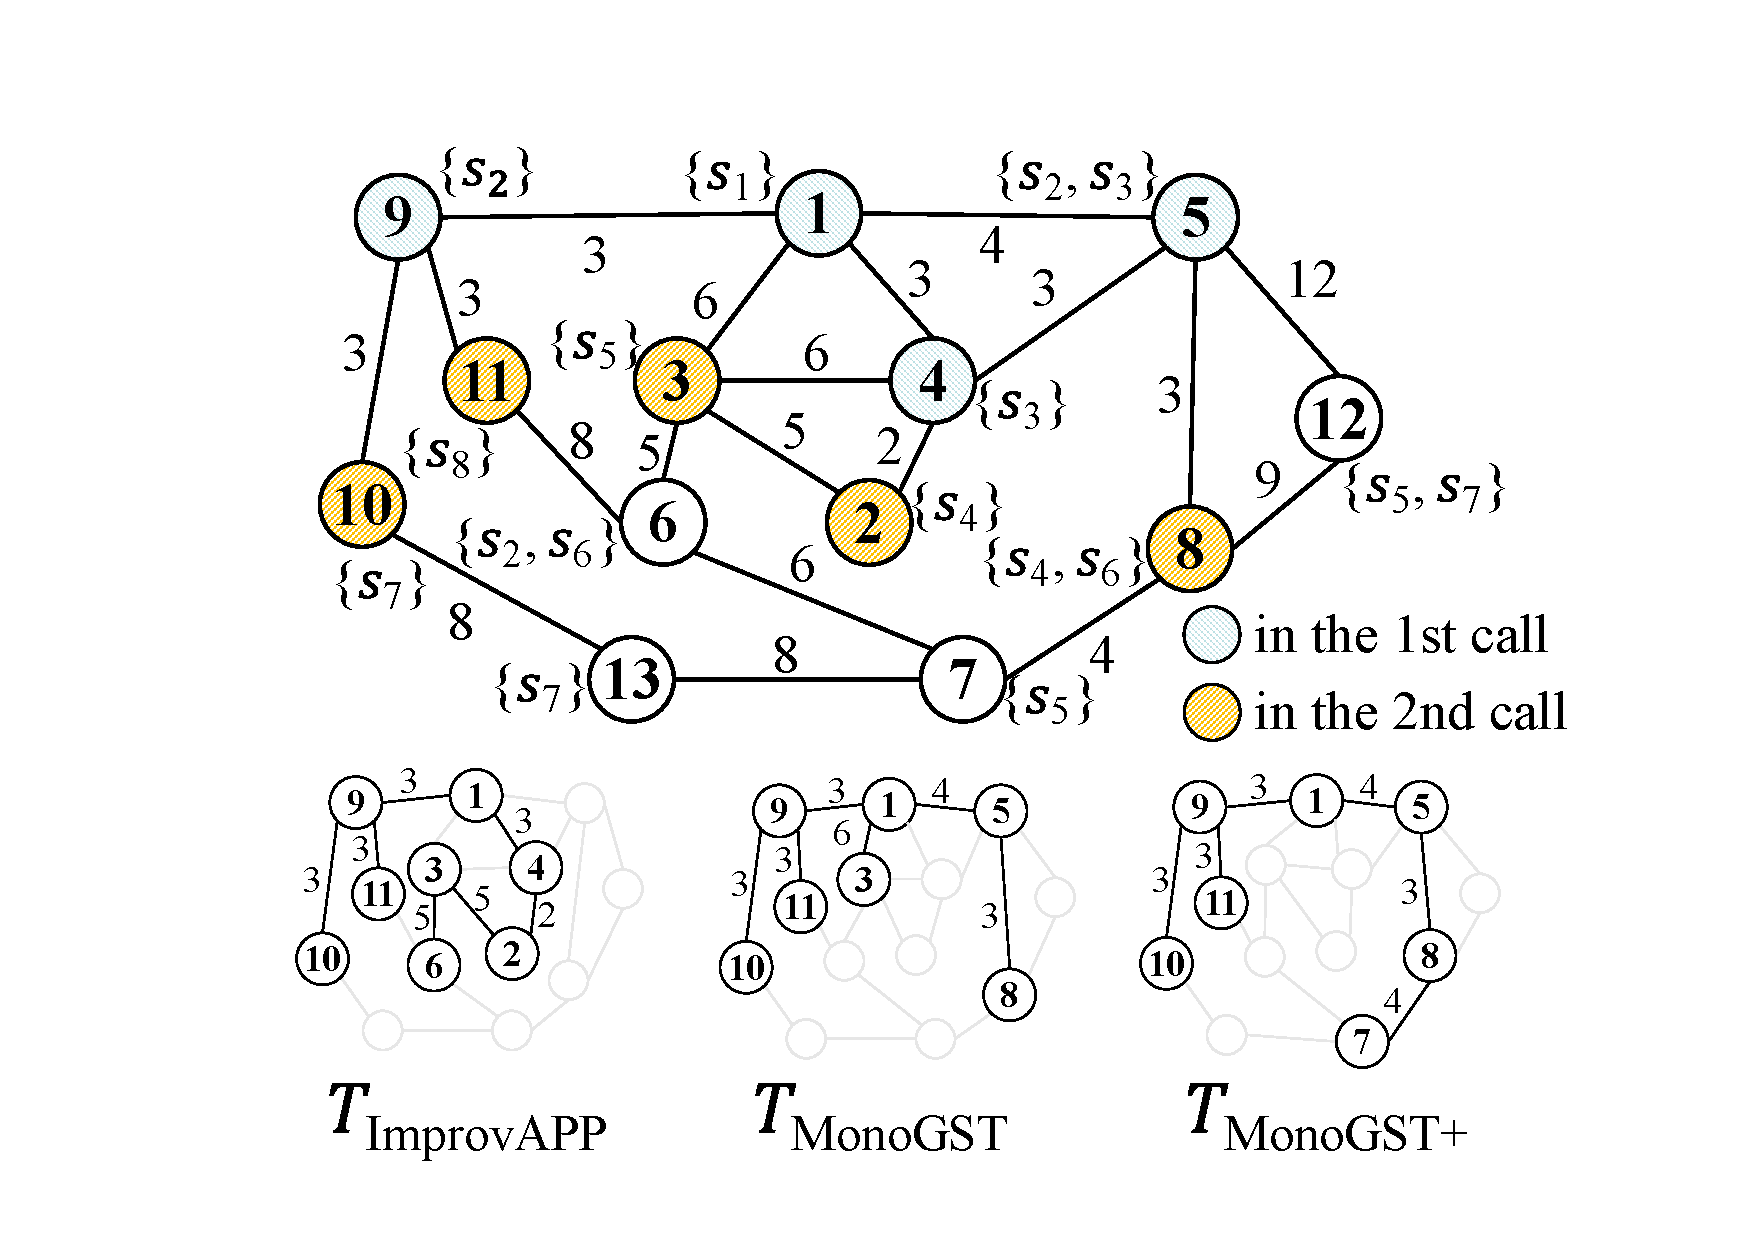
\includegraphics[width=\linewidth]{fig/application/ill7.pdf}%
      \label{fig:TF}%
    }
  \end{minipage}\hfill
  \begin{minipage}[t]{0.32\textwidth}
    \centering
    \subfloat[Consider a technology-themed KG, along with an illustrative query ``Apple Innovation Expo California.'' For this query, each keyword is mapped to a group of entity vertices in the KG: $\textit{Apple}\mapsto \{\#1,\#2\}$, $\textit{Innovation}\mapsto \{\#7,\#8\}$, $\textit{Expo}\mapsto \{\#7,\#10\}$, and $\textit{California}\mapsto \{\#4,\#11\}$. The dashed-boxed subgraph~$T$ is a feasible answer to this query; this GST simultaneously covers and connects all the four keyword-induced groups. \label{fig: KS}]{%
      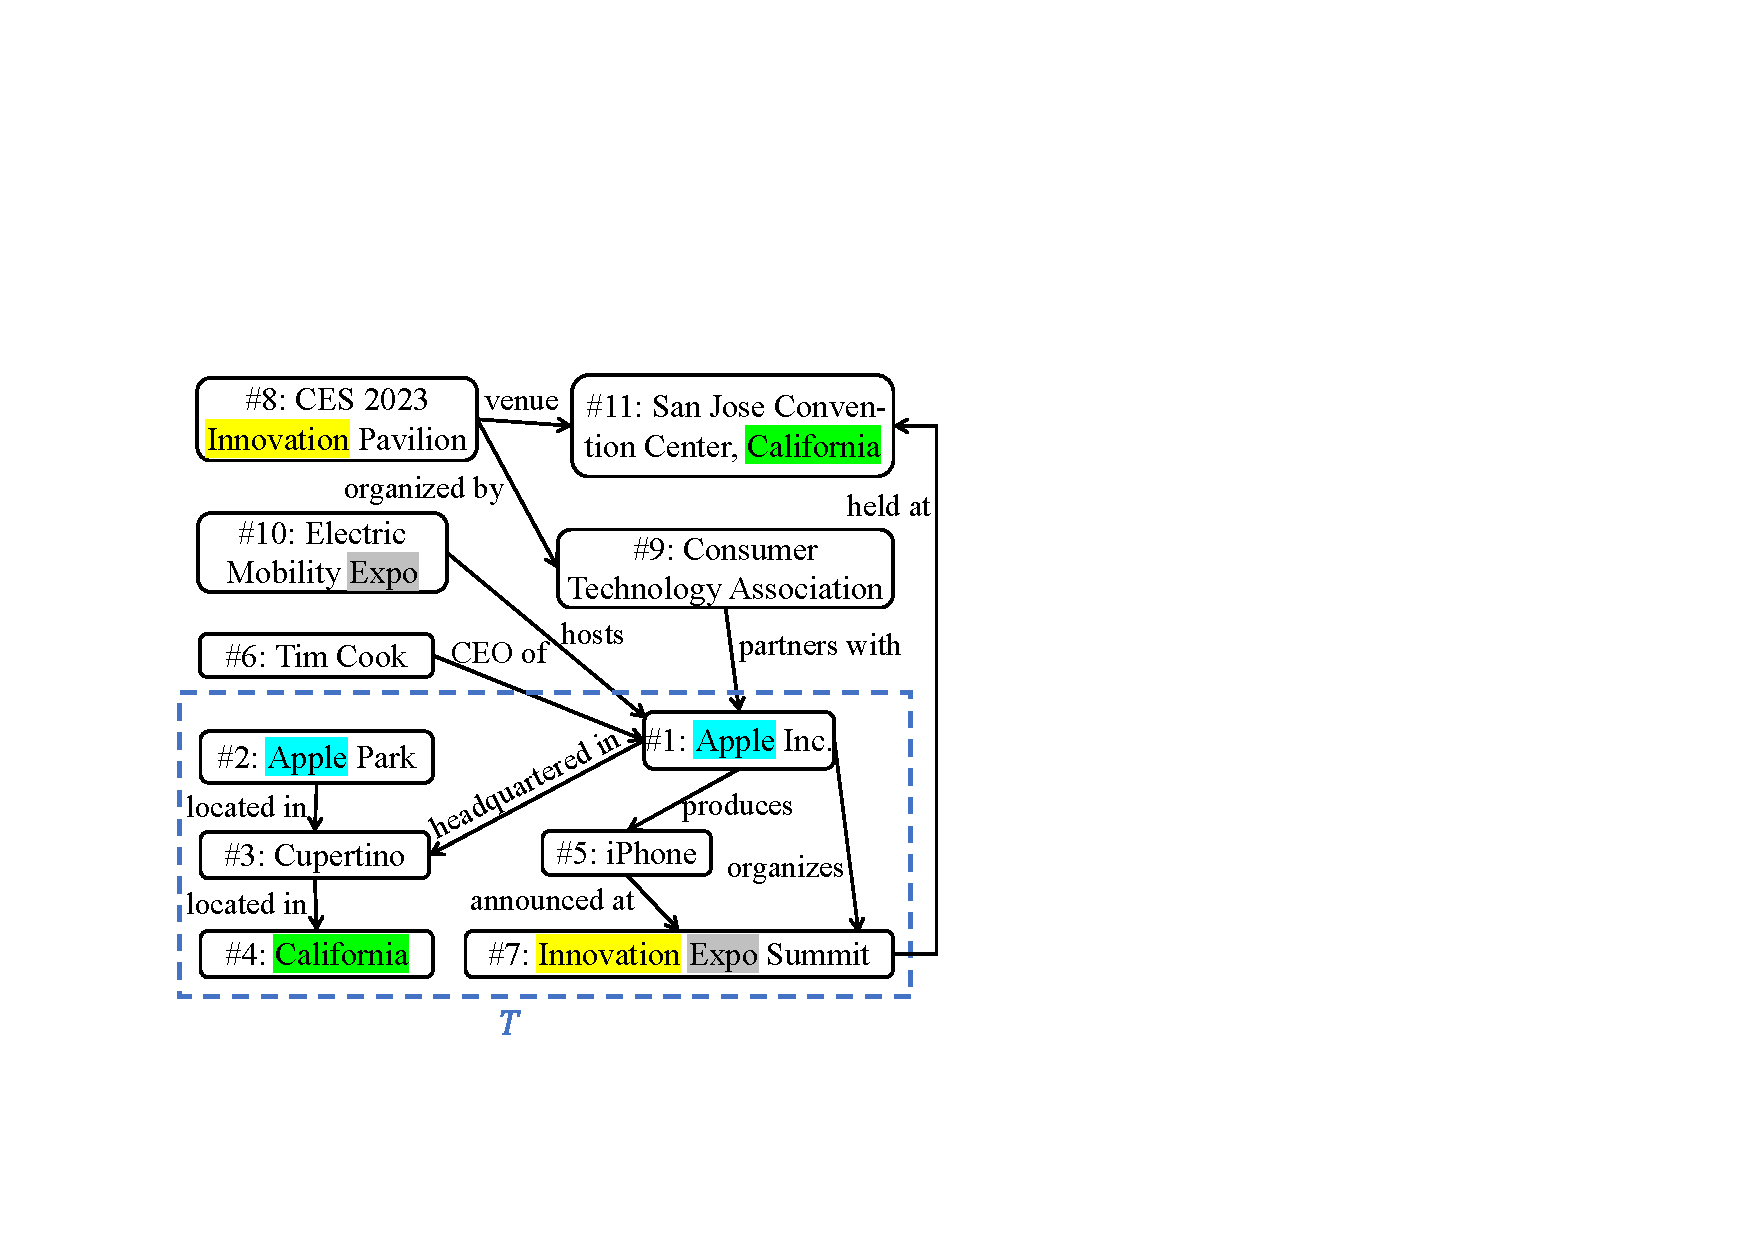
\includegraphics[width=\linewidth]{fig/application/pic2b.pdf}%
      \label{fig:KS}%
    }
  \end{minipage}
  \hfill
  \begin{minipage}[t]{0.314\textwidth}
    \centering
    \subfloat[The top part is a KG; vertices (or edges) with the same color have the same EDP (or LP) and form a group. Subdividing the colored edges by inserting vertices and removing classes (dotted boxes) and literals (quoted) yields an ELG in the bottom part. The dashed-boxed GST~$T$ covers all pattern-induced groups. Extending it back to a subgraph of the original KG by restoring the removed classes and literals, we will obtain a feasible pattern-coverage summary. \label{fig: KGS}]{%
      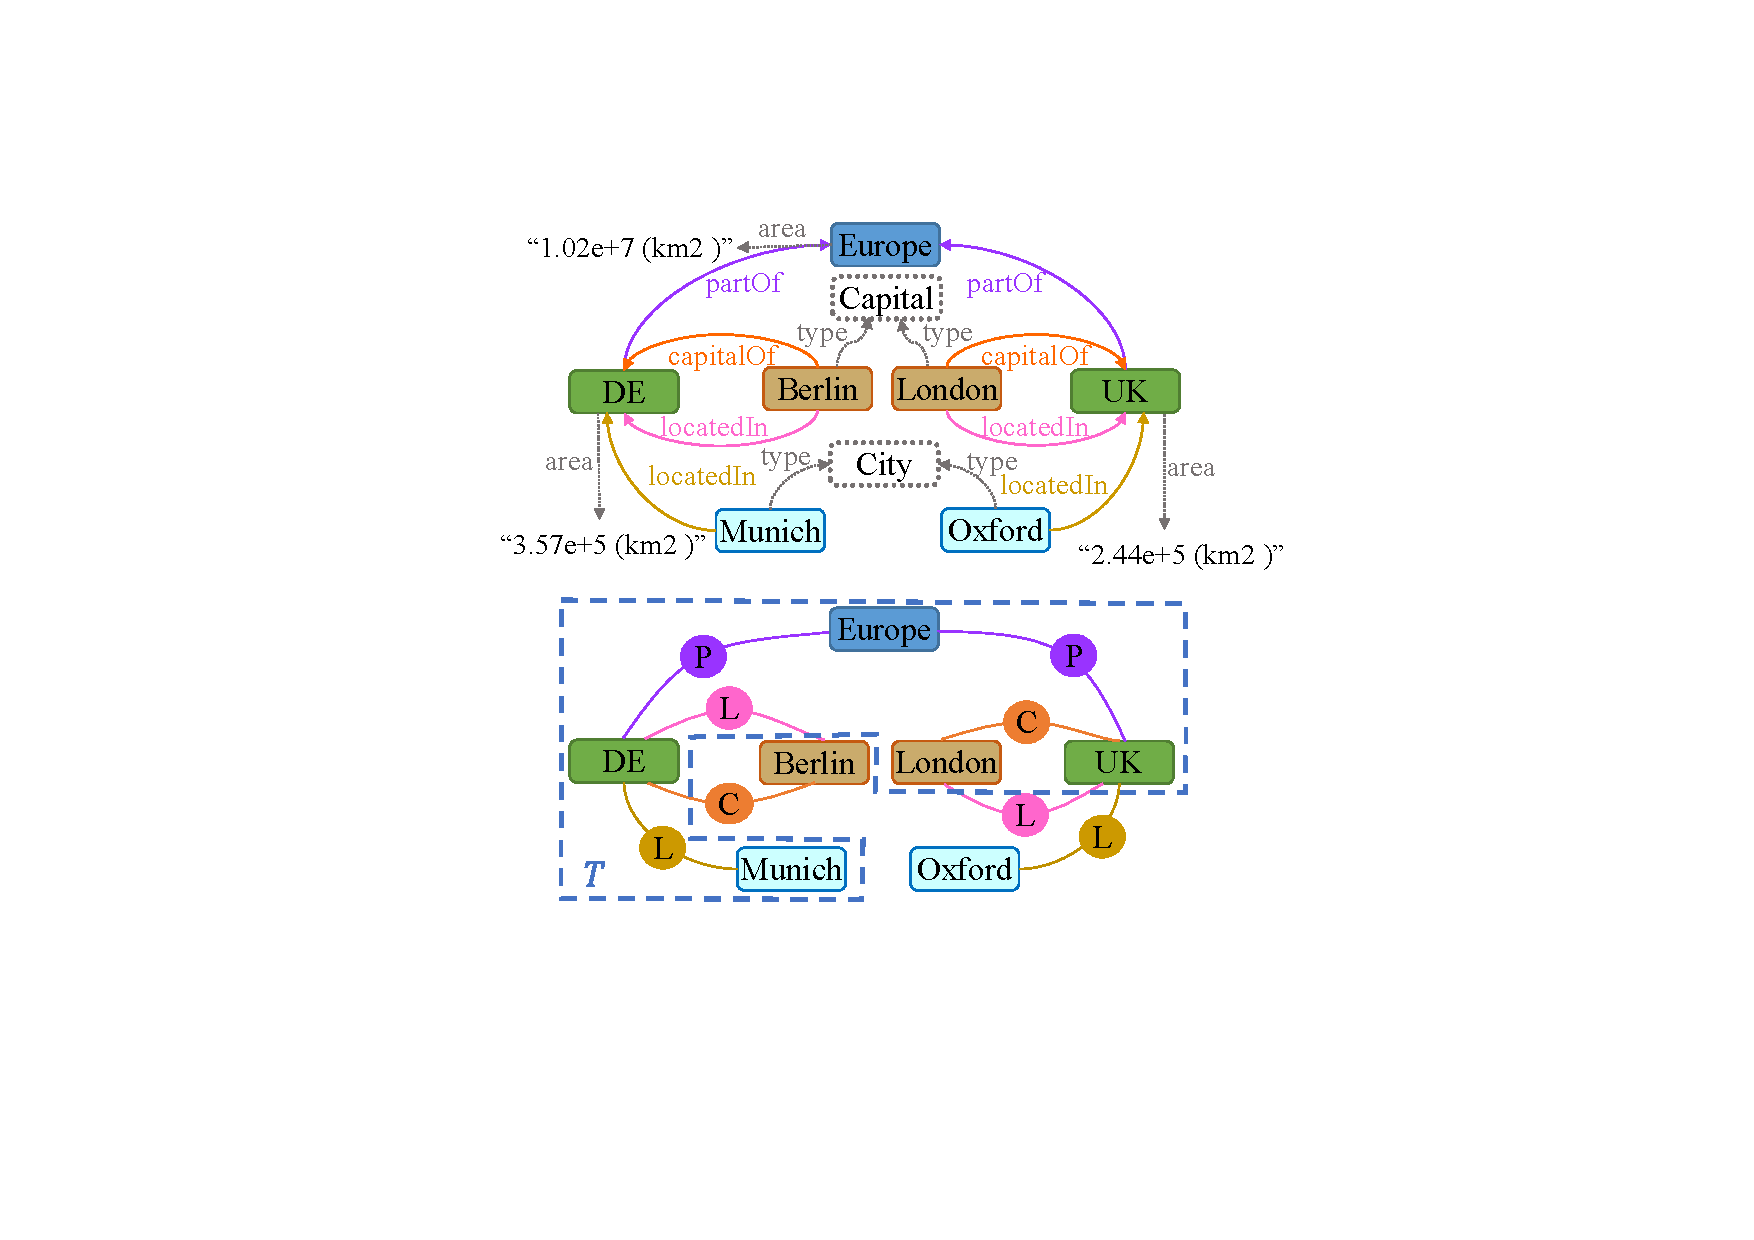
\includegraphics[width=\linewidth]{fig/application/pic3c.pdf}%
      \label{fig:KGS}%
    }
  \end{minipage}

  % \vspace{1ex}

  % % ===== Row 2: three columns (KGS_1 | (KGS_2 over KGS_3) | KGS_4) =====
  % \begin{minipage}[t]{0.372\textwidth}
  %   \centering
  %   \subfloat[An example of RDF Dataset, vertices or edges with the same color indicate that they belong to the same type. \label{fig: KGS_1}]{%
  %     \includegraphics[width=\linewidth]{fig/application/KGS1_.pdf}%
  %     \label{fig:KGS1}%
  %   }
  % \end{minipage}\hfill
  % \begin{minipage}[t]{0.27\textwidth}
  %   \centering
  %   \subfloat[The Entity-Link Graph (ELG) converted from RDF and a feasible GST covering all types in the ELG. \label{fig: KGS_23}]{%
  %     \includegraphics[width=\linewidth]{fig/application/KGS23.pdf}%
  %     \label{fig:KGS1}%
  %   }
  % \end{minipage}\hfill
  % \begin{minipage}[t]{0.34\textwidth}
  %   \centering
  %   \subfloat[Extend the GST to obtain the Pattern-Coverage Snippet. \label{fig: KGS_4}]{%
  %     \includegraphics[width=\linewidth]{fig/application/KGS4.pdf}%
  %     \label{fig:KGS4}%
  %   }
  % \end{minipage}

  \caption{Application scenarios of GSTP.}
  \label{fig: application}
\end{figure*}

% Convert each RDF edge into a vertex and remove gray types and literals to obtain an Entity-Link Graph (ELG). Next, in the ELG, find a minimum subgraph that covers all types; each type corresponds to a set of vertices, so this can be solved via GST. The figure above shows the ELG corresponding to Fig.~\ref{fig: KGS_a} and a valid subgraph of this ELG that covers all types.

\textbf{Application Scenarios.}
GSTP finds applications in the following representative scenarios in graph data management and mining.

\textit{Team Formation.} In social networks,
\iffalse~\cite{TF_3}\fi
vertices represent experts annotated with skills, edges encode acquaintance or collaboration, and smaller edge weights indicate closer relationships. Expert team formation~\cite{TF_4, TF_5} requires the selection of a team of experts whose collective skills cover a specified set while maintaining strong connectivity. In GSTP-based solutions~\cite{TF_3\iffalse TF_1\fi, ImprovAPP}, each required skill corresponds to a group of experts who possess that skill, and a small-weight GST corresponds to a cohesive team. See Figure~\ref{fig: TF}.

\textit{Keyword-Based Exploration.} In knowledge graphs (KGs)~\cite{KG_D}, entities are vertices, and relations are edges; relational databases are converted into graphs where tuples are vertices and foreign keys are edges, often weighted. Keyword-based exploration~\cite{KS_3,\iffalse KS_2\fi KS_1} helps users extract relevant structures. GSTP-based solutions~\cite{KS_6, KS_7\iffalse KS_4\fi, KS_5} map each input keyword to a group of matching vertices and return a minimum-weight tree covering all groups. See Figure~\ref{fig: KS}.

\textit{Knowledge Graph Summarization.} To reuse a KG, its summary~\cite{KS_3, KGS_3} provides users with an overview of its core content. The state-of-the-art Pattern-Coverage Snippet Generation (PCSG) method~\cite{KGS_1} builds an Entity-Link Graph (ELG) from a KG and uses Entity Description Pattern (EDP) and Link Pattern (LP) to classify entities and relations into groups, respectively. This GSTP-based solution induces an optimal summary with the greatest compression from a smallest subgraph of the ELG showing all patterns. See Figure~\ref{fig: KGS}.

\textit{Very-Large-Scale Integration.} In integrated circuit design, min-cost routing~\cite{VLSI_3} connects multiple equivalent pins. GSTP-based solutions~\cite{VLSI_1, VLSI_2} run on the Hanan grid reduction of a circuit net.

% \textit{Pathway Discovery in Metabolic Networks.} In computational biology, identifying metabolic pathways can be modeled as GSTP~\cite{PI}, illustrating an interdisciplinary application.

\textbf{Motivation.} GSTP is NP-hard~\cite{ProveNP}. Exact algorithms such as DPBF~\cite{KS_5} and PrunedDP++~\cite{PrunedDP} have an exponential running time in the number of groups~$g$ and are difficult to scale to large graphs. This motivates \emph{practical approximation algorithms}. The state of the art includes ImprovAPP~\cite{ImprovAPP} and the index-based KeyKG$^+$~\cite{KeyKG}.
% using a distance oracle~\cite{HL_INTRO} for shortest-path queries and requiring substantial preprocessing time.
They guarantee a $(g-1)$ approximation, i.e., an approximation ratio linear in~$g$. Earlier algorithms such as BANKS~\cite{BANKS}, BANKS-II~\cite{BANKS2}, and BLINKS~\cite{BLINKS} also provide $O(g)$-approximation guarantees.
% but tend to be less efficient on large graphs~\cite{KeyKG}.
All these approaches are inspired by the so-called 1-star structure~\cite{gsub1_source}.

For a \emph{more accurate approximation}, PartialOPT~\cite{ImprovAPP} achieves a $(g-h+1)$ approximation with a parameter $h$, but its running time grows exponentially with~$h$. There are also algorithms with polylogarithmic approximation ratios~\cite{PolyAppr_1, PolyAppr_2}, embedding the graph into a tree metric to solve. However, they are primarily of theoretical interest.
% and become inefficient for large graphs, e.g.,~relying on linear programming (LP) solvers.
Besides, while using the $d$-star structure has the potential to produce a ratio sublinear in~$g$, experimental validation is lacking for large graphs, e.g.,~the 2-star heuristic~\cite{dstar1,dstar2} requiring expensive all-pairs shortest path computation, and the reduction to the Directed Steiner Tree Problem (DSTP)~\cite{D_STP}.

\emph{In summary, existing practical methods typically have mediocre (\dew{i.e.,}~linear) approximation guarantees, while methods with stronger (\dew{i.e.,}~sublinear) guarantees still lack scalability validation.} Table~\ref{table: Algorithms Comparison} summarizes their time complexities and approximation ratios.

\textbf{Our Work.}
To bridge this performance trade-off, our goal is to develop a practical GST algorithm that is \emph{both effective}, providing a sublinear approximation guarantee, \emph{and efficient}, with a speed on par with the fastest index-free linear-approximation algorithms.

% Section~\ref{sec: preliminaries} formulates GSTP and reviews the 2-star structure. Section~\ref{sec: basic}
Specifically, we first propose a basic two-step algorithm \BasicPTS, which greedily approximates via 2-star based on distances calculated by Dijkstra's algorithm and non-trivially achieves an approximation ratio $O(\sqrt g)$.
% In Section~\ref{sec: improved},
Our improved algorithm \ImprovPTS incorporates a \emph{suspendable Dijkstra's algorithm} to calculate distances as needed, leverages the \emph{monotonicity and unimodality of the greedy function} to prune the search space, and constructs a GST from a 2-star through \emph{a greedy re-selection of paths} to enhance the approximation.
% Section~\ref{sec: experiments} empirically demonstrates the efficiency and effectiveness of our approach in multiple scenarios. Finally, Section~\ref{sec: relatedwork} discusses related work and Section~\ref{sec: conclusion} concludes the paper.
Our technical contributions are as follows.
\begin{itemize}
  \item For \BasicPTS, which greedily solves a weighted set cover problem to approximate an optimum 2-star and converts it into a GST, we perform a holistic analysis of this two-step approximation, producing a guaranteed ratio of $O(\sqrt g)$.
  \item In \ImprovPTS, we embed the set cover procedure within Dijkstra's algorithm to establish a dynamic bounding mechanism and exploit the monotonicity and unimodality of the greedy function, substantially pruning the search space.
\end{itemize}
% \textbf{Motivation.} Because the problem is NP-Hard, research on efficient algorithms focuses on approximation algorithms. In the past, Most of the work can not take into account both the practical operation and theoretical approximation ratio. For example, in recent years, algorithms such as KeyKG ~\cite{DBLP:conf/www/Shi0K20} using index and ImprovAPP and PartialOPT ~\cite{DBLP:journals/pvldb/SunX0HL021} without index have an approximate ratio of around $g-1$.

% However, some algorithms with good theoretical approximation, their actual running speed will be unsatisfactory. For example, 2-star ~\cite{DBLP:conf/date/HelvigRZ98,DBLP:conf/ispd/BatemanHRZ97} algorithm does not have enough space to index $O(1)$ time-cost queries on large graphs, and its own running speed is very complex with respect to $n$ and $g$, and the actual running speed is also very slow. Other algorithms based on linear programming and rounding, such as polylogarithmic-approximation algorithm ~\cite{DBLP:journals/jal/GargKR00}, but are also obviously not feasible to run on actual large graphs. 

% Therefore, an algorithm that has a lower approximation ratio of linear theory about g and can run on real graphs is needed.

% \textbf{Our work.} In this paper, we propose new efficient sublinear approximation ratio algorithms based on 2-star method, which also has $O(\sqrt{g}\ln{g})$ approximation ratio. We reexamine the problem from the perspective of set coverage, and give new weight functions and property derivations. Based on the weight function, we carry out a series of pruning, which greatly improves the actual operation efficiency of the algorithm. \shan{TODO}

\begin{table}[t]
    \centering
    \caption{Comparison between GST algorithms.}
    \label{table: Algorithms Comparison}
    \resizebox{\linewidth}{!}{
    \begin{tabular}{lrr}
        \toprule
        Algorithm & Time Complexity & Approx. Ratio \\
        \midrule
%        \multicolumn{3}{l}{\emph{Exact algorithms:}}\\
%        DPH & $O(3^g*n^2+2^gnm)$ & $1$\\
        DPBF & $O(3^gn+2^g((g+\log{n})n+m))$ & $1$\\
        PrunedDP$++$ & $O(3^gn+2^g((g+\log{n})n+m))$ & $1$\\
        \hline
%        \multicolumn{3}{l}{\emph{Sublinear-approximation algorithms:}}\\
        Reduction to tree metric & polynomial & $O(\log ^3n\log g)$\\
        % \gong{Modified-GS} & dependent on LP solvers & $O(\log ^3n\log g)$ \\
        \Basic (ours) & $O(n(m+ng^2+n\log n))$ & $O(\sqrt g)$\\
        \ImprovPTS (ours) & $O(n(m+(n+g)g+n\log n))$ & $O(\sqrt g)$\\
         Reduction to DSTP  & $O(n(mg+ng\log n))$ & $O(\sqrt g)$ \\
         2-star heuristic & $O(n^3+n^2g^2)$ & $O(\sqrt g\ln g)$\\ 
        \hline
%        \multicolumn{3}{l}{\emph{Linear-approximation algorithms:}}\\
        PartialOPT & $O(n(gn+3^hn+2^h(m+hn+n\log{n})))$ & $g-h+1$\\
        KeyKG$^+$ & $O(n^2g+ng^3)$ & $g-1$\\
        ImprovAPP & $O(g(m+n\log{n}+n^2+n\log{g}))$ & $g-1$ \\
        BANKS & $O(n^2\log{n}+nm)$ & $O(g)$\\
        BANKS-II & $O(n^2\log{n}+nm)$ & $O(g)$\\
        BLINKS & dependent on partition & $O(g)$\\
        \bottomrule
    \end{tabular}
    }
\end{table}

Experiments on five diverse real-world datasets demonstrate that \ImprovPTS attains better solution quality than existing approximation algorithms while running as fast as the state-of-the-art index-free linear-approximation solver, thereby bridging the long-standing effectiveness-efficiency trade-off in GSTP research.